\documentclass[11pt, french, aspectratio=32]{beamer}

\usepackage{soutenance}

\AtBeginDocument{%
  \bookmark[named=FirstPage, level=subsection]{Title frame}%
}

\title{%
  Impact des Fronts sur le Phytoplancton\\
  dans la Région du Gulf Stream\\
  Quantifié par Imagerie Satellitaire
}

\author{Clément Haëck}

\direction{Marina Lévy et Laurent Bopp}

\institute{%
  Laboratoire d'Océanographie et du Climat\\Expérimentations et Analyses Numériques
}

\begin{document}

%% Title frame --------------------------
{
  \usebackgroundtemplate{
    \parbox[t][\paperheight]{\paperwidth}{
    \vfill\par
    \hfill
    \includegraphics[width=0.7\paperwidth, height=0.7\paperheight, keepaspectratio]{title_background.jpg}}
  }
  \begin{frame}[plain, noframenumbering]
    \titlepage%
  \end{frame}
}

\section*{Introduction}
\subsection{Le phytoplancton}

%% --------------------------------------

\begin{frame}
  \frametitle{Qu'est-ce que le phytoplancton ?}
  {%
    \includegraphics[
    width=\textwidth, height=0.9\textheight, keepaspectratio
    ]{patchwork.pdf}%
    \centering%
  }%
\end{frame}

%% --------------------------------------

\begingroup
\newcommand\graph[2]{%
    \llap{\includegraphics<#2>[
    width=\textwidth, height=0.9\textheight, keepaspectratio
    ]{_intro_verticale/#1<#2>.pdf}}}%
\begin{frame}
  \frametitle{Contrôles de la croissance du phytoplancton}
  {
    \centering
    \includegraphics[
    width=\textwidth, height=0.9\textheight, keepaspectratio
    ]{_intro_verticale/base<1->.pdf}%
    \graph{photosynthese}{1-4}%
    \graph{euphotique}{2-}%
    \graph{nutriments}{3-}%
    \graph{melange}{4-}%
    \graph{echanges}{5-}%
  }
\end{frame}
\endgroup

%% --------------------------------------

\begin{frame}
  \frametitle{Exemple de bloom}
  \includegraphics<1>[
  width=\linewidth, height=0.8\textheight, keepaspectratio
  ]{true_color_0527.jpg}%
  \includegraphics<2>[
  width=\linewidth, height=0.92\textheight, keepaspectratio
  ]{true_color_0527_zoom.jpg}%
  \\
  {\small
    27 mai 2023, données L1 MODIS-Aqua
  }
\end{frame}

%% --------------------------------------

\begin{frame}
  slide d'explication couleur chlorophylle-a,

  sinon juste à l'oral
\end{frame}

%% --------------------------------------

\begin{frame}[label=chlsnapshot]
  \frametitle{Répartition horizontale du phytoplancton}
  \begin{beamercolorbox}[sep=0pt, right]{}
    \includegraphics[height=0.8\textheight]{chl_snapshot_GS.pdf}
    \\
    {\footnotesize Chlorophylle-a L2 MODIS-Terra, 23 février 2020}
  \end{beamercolorbox}
\end{frame}

%% --------------------------------------

\begingroup
\newcommand\graph[2]{%
    \llap{\includegraphics<#2>[
    width=\textwidth
    ]{_levy_2023_fig1/#1<#2>.pdf}}}%
\begin{frame}
  \frametitle{Observer le phytoplancton}
  {
    \centering
    \includegraphics[width=\textwidth]{_levy_2023_fig1/base<1->.pdf}%
    \graph{grids}{3-}%
    \graph{sat}{4}%
    \graph{insitu}{2-}%
  }

  \begin{itemize}
    \item<2-> Mesures in-situ
    \item<3-> Modèles numériques biogéochimiques
    \item<4-> \emph{Images satellites}
  \end{itemize}
\end{frame}
\endgroup

%% --------------------------------------

\subsection{Influence des courants}

\begin{frame}
  \frametitle{Influence des courants: Grande échelle}
  \includegraphics<1>[
    width=\textwidth, height=0.85\textheight, keepaspectratio
  ]{chl_month_avg.pdf}
  \includegraphics<2>[
    width=\textwidth, height=0.85\textheight, keepaspectratio
  ]{nutriments_global.pdf}
\end{frame}

%% --------------------------------------

\againframe<2>{chlsnapshot}

%% --------------------------------------

\begingroup
\newcommand\graph[2]{%
  \llap{\includegraphics<#2>[height=0.75\textheight]{_front_circulation/#1<#2>.pdf}}}%
\begin{frame}<1-5>[label=frontogenese]
  \frametitle{Frontogénèse et remontée des nutriments}
    \includegraphics[height=0.75\textheight]{_front_circulation/base<1->.pdf}%
    \graph{upwell}{5}%
    \graph{isopycnals}{1-}%
    \graph{jet}{2-}%
    \graph{vorticity}{3-}%
    \graph{circulation}{4-}%
    \graph{mld}{6}%
\end{frame}

%% --------------------------------------

\begin{frame}
  \frametitle{Quantification de l'apport de nutriments}

  littérature

\end{frame}

%% --------------------------------------

\againframe<6>{frontogenese}
\endgroup

%% --------------------------------------

\begin{frame}
  \frametitle{Modification de la phénologie du bloom}
  seulement dans un modèle (même si forcé par observations)

  \begin{block}{}
    \includegraphics[width=0.4\textwidth]{mahadevan_2012_fig3.pdf}
    \\
    Mahadevan et al.\ (2012)
  \end{block}
\end{frame}

%% --------------------------------------

\subsection{Problématiques}

\begin{frame}
  \boxtitle{Problématiques}
  \vspace{2em}

  \begin{beamercolorbox}[sep=0pt]{}
    \begin{enumerate}
      \setlength{\itemsep}{1.2em}
      \item Comment quantifier la \emph{réponse de la chlorophylle-a} aux dynamiques \emph{frontales}
      \item<2-> Influence de la \emph{saison}, du \emph{régime} biogéochimique, et de \emph{l’intensité} des fronts ?
      \item<3-> Détecter un \emph{bloom précoce} dans les fronts ?
    \end{enumerate}
  \end{beamercolorbox}
\end{frame}

%% --------------------------------------

\begingroup
\newcommand\graph[2]{%
    \llap{\includegraphics<#2>[
    width=\textwidth, height=0.9\textheight, keepaspectratio
    ]{_region_etude/#1<#2>.pdf}}}%
\begin{frame}
  \frametitle{Région d'étude: autour du Gulf Stream}
  \includegraphics[
  width=\textwidth, height=\textheight, keepaspectratio
  ]{_region_etude/base_chl<1->.pdf}%
  \graph{base_sst}{1-7}%
  \graph{gulfstream}{2-7}%
  \graph{gyre}{3-7}%
  \graph{talus}{4-7}%
  \graph{subtrop_perm}{5-}%
  \graph{subpol}{6-}%
  \graph{subtrop_sais}{7-}%
  \graph{problematiques}{8-}%
\end{frame}
\endgroup

%% --------------------------------------

\section*{Méthodes - Détection des fronts}

\begin{frame}
  \boxtitle{Méthodes - Détection des fronts}
\end{frame}

%% --------------------------------------

\begin{frame}
  \frametitle{Détecter les fronts par satellite}

  \begin{block}{}
    On utilise la \strong{SST} comme proxy de la densité
  \end{block}

  \begin{block}{}
    Plusieurs méthodes existantes:
    \begin{itemize}
            \setlength{\itemsep}{1.2em}
      \item “simple” dérivation: gradient, Sobel, Laplacien, \dots
      \item filtrer auparavant: Canny (1986), Belkin--O'Reilly (2009)
      \item fenêtre glissante: Cayula--Cornillon (1992), Nieto et al. (2012), Miller (2009), \strong{Liu \& Levine (2016)}
    \end{itemize}
  \end{block}
\end{frame}

%% --------------------------------------

\begin{frame}
  \frametitle{Méthode du “Heterogeneity-index”}
  \onslide<1->{Fenêtre glissante}\onslide<2->{, dans laquelle on calcule 3 composantes}
  \\[1em]
  \multigraphtrans[height=0.75\textheight]{4}{zoom_front}
\end{frame}

%% --------------------------------------

\begin{frame}
  \frametitle{Données utilisées: SST}

  \begin{block}{Choisie dans la suite}
    \begin{itemize}
      \item ESA-SST-CCI / C3S
      \item journalières, 4km
      \item L4: interpolation spatiale de multicapteurs IR, pas de nuages
    \end{itemize}
  \end{block}

  \vfill

  \includegraphics[height=0.5\textheight]{comparaison_sst.pdf}

\end{frame}

\begin{frame}
  \frametitle{Données utilisées: Chl-a}

  \begin{block}{Choisie dans la suite}
    \begin{itemize}
      \item Copernicus-Globcolour,
      \item journalières, 4km
      \item L3: multicapteurs, avec nuages
    \end{itemize}
  \end{block}

  \vfill

  \includegraphics[height=0.5\textheight]{comparaison_chl.pdf}

\end{frame}

%% --------------------------------------

\begingroup
\newcommand\graphstep[2]{%
  \llap{\includegraphics<#2>[width=\textwidth]{_exemple_front/#1<#2>.pdf}}}%
\begin{frame}
  \frametitle{Exemple de front}
  \includegraphics[width=\textwidth]{_exemple_front/base<1->.pdf}%
  \graphstep{SST}{1-}%
  \graphstep{composantes}{2-6}%
  \graphstep{arrows_out}{3-6}%
  \graphstep{hi_image}{3}%
  \graphstep{hi_real_image}{4-}%
  \graphstep{HI_axes}{3-}%
  \graphstep{hi_title}{3}%
  \graphstep{hi_real_title}{4-}%
  \graphstep{xlabels}{3}%
  \graphstep{xlabels_real}{4-}%
  \graphstep{contours_colorbar}{5-}%
  \graphstep{contours}{5-}%
  \graphstep{contours_compo}{6}%
  \graphstep{contours_sst}{6-}%
  \graphstep{chla}{7-}%
\end{frame}
\endgroup

%% --------------------------------------

\section{Région subtropicale -- Augmentation de la Chlorophylle dans les fronts}
\begingroup
\newcommand\graph[1]{%
    \llap{\includegraphics[
    width=\textwidth, height=0.9\textheight, keepaspectratio
    ]{_region_etude/#1.pdf}}}%
\begin{frame}
  \boxtitle{Partie 1}

  \includegraphics[
  width=\textwidth, height=\textheight, keepaspectratio
  ]{_region_etude/base_chl<1->.pdf}%
  \graph{subtrop_perm<5->}%
  \graph{subtrop_sais<7->}%
  \graph{subpol<6->}%
  \graph{problematiques<8->}%
  \graph{blocker_2}%
  \graph{blocker_3}%
\end{frame}
\endgroup

%% --------------------------------------

\begingroup
\newcommand\graphstep[2]{%
  \llap{\includegraphics<#2>[
    width=\textwidth, height=0.9\textheight, keepaspectratio
    ]{_distrib_region_perm/#1<#2>.pdf}}}%
\begin{frame}
  \frametitle{Mesure de l'impact des fronts}
  \includegraphics[
    width=\textwidth, height=0.9\textheight, keepaspectratio
  ]{_distrib_region_perm/base<1->.pdf}%
  \graphstep{front_mask}{2-}%
  \graphstep{base_top}{1-}%
  \graphstep{histogram}{3-}%
  \graphstep{hist_back}{4-}%
  \graphstep{hist_fronts}{3-}%
\end{frame}
\endgroup

%% --------------------------------------

\begingroup
\newcommand\graphstep[2]{%
  \llap{\includegraphics<#2>[height=0.8\textheight]{_res_perm/#1<#2>.pdf}}}%
\begin{frame}
  \frametitle{Résultats}
  \includegraphics[height=0.8\textheight]{_res_perm/base<1->.pdf}%
  \graphstep{top_xlabels_med}{1-4}%
  \graphstep{med_one_year}{1}%
  \graphstep{med_all_years}{2}%
  \graphstep{med_cli}{3-}%
  \graphstep{top_xlabels_exces}{4}%
  \graphstep{exces}{4-}%
  \graphstep{surface}{5-}%
  \graphstep{surplus}{6-}%
\end{frame}
\endgroup

%% --------------------------------------

\begin{frame}
  \frametitle{Conclusion partie 1}
  \begin{minipage}{0.85\linewidth}
    \begin{itemize}
            \setlength{\itemsep}{3em}
      \item détection d'une augmentation locale de la Chl-a~(\pct{\approx 40})
      \item moins important que précédemment mesuré\\(Liu \& Levine 2016,~\pct{\approx 80})
      \item effet global moindre lorsque l'on prend en compte la surface impactée~(\pct{\approx 3})
    \end{itemize}
  \end{minipage}
\end{frame}

%% --------------------------------------

\section{Région du Gulf-Stream -- Intensité des fronts}
\begingroup
\newcommand\graph[1]{%
    \llap{\includegraphics[
    width=\textwidth, height=0.9\textheight, keepaspectratio
    ]{_region_etude/#1.pdf}}}%
\begin{frame}
  \boxtitle{Partie 2}

  \includegraphics[
  width=\textwidth, height=\textheight, keepaspectratio
  ]{_region_etude/base_chl<1->.pdf}%
  \graph{subtrop_perm<5->}%
  \graph{subtrop_sais<7->}%
  \graph{subpol<6->}%
  \graph{problematiques<8->}%
  \graph{blocker_1}%
  \graph{blocker_3}%
\end{frame}
\endgroup

%% --------------------------------------

\begingroup
\newcommand\graph[2]{%
  \llap{\includegraphics<#2>[
    width=\textwidth, height=0.8\textheight, keepaspectratio
    ]{_zone_separation/#1<#2>.pdf}}}%
\begin{frame}
  \frametitle{Découpage en sous-régions}
  \includegraphics[
  width=\textwidth, height=0.8\textheight, keepaspectratio
  ]{_zone_separation/base<1->.pdf}%
  \graph{hist_in}{1-2}%
  \graph{fit_gauss}{2}%
  \graph{separation}{3-}%
\end{frame}
\endgroup

%% --------------------------------------

\begin{frame}
  \frametitle{Évolution de la Chl-a avec le HI}
  \includegraphics[
  width=\textwidth, height=0.8\textheight, keepaspectratio
  ]{results/chl_vs_hi.pdf}
\end{frame}

%% --------------------------------------

\begin{frame}
  \frametitle{Occurence des fronts}
  \begin{overlayarea}{\textwidth}{0.25\textheight}
    \centering
    \includegraphics<1>{fronts_delineation.pdf}
    \only<2>{
      \vspace{1em}
      \begin{minipage}{0.45\textwidth}
        \centering
        fronts faibles:\\ submésoéchelle, éphémères
      \end{minipage}
      \hfill
      \begin{minipage}{0.45\textwidth}
        \centering
        fronts forts:\\ mésoéchelle, permanents
      \end{minipage}
    }
    \\
  \end{overlayarea}

  \vfill

  \includegraphics[
  width=\textwidth, height=0.75\textheight, keepaspectratio
  ]{results/fronts_occurrence.pdf}

\end{frame}

%% --------------------------------------

\begin{frame}
  \frametitle{Climatologies}
  \includegraphics[
  width=\textwidth, height=0.8\textheight, keepaspectratio
  ]{results/ts_climatology.pdf}
\end{frame}

%% --------------------------------------

\begin{frame}
  \frametitle{Conclusion partie 2}

  \vfill
  \begin{itemize}
    \setlength{\itemsep}{\stretch{1}}
    \item yeah
  \end{itemize}
  \vfill

\end{frame}

%% --------------------------------------

\section{Région subpolaire -- Phénologie du bloom}
\begingroup
\newcommand\graph[1]{%
    \llap{\includegraphics[
    width=\textwidth, height=0.9\textheight, keepaspectratio
    ]{_region_etude/#1.pdf}}}%
\begin{frame}
  \boxtitle{Partie 3}

  \includegraphics[
  width=\textwidth, height=\textheight, keepaspectratio
  ]{_region_etude/base_chl<1->.pdf}%
  \graph{subtrop_perm<5->}%
  \graph{subtrop_sais<7->}%
  \graph{subpol<6->}%
  \graph{problematiques<8->}%
  \graph{blocker_1}%
  \graph{blocker_2}%
\end{frame}
\endgroup

%% --------------------------------------

\begin{frame}
  \frametitle{Chronométrer le bloom: démarrage et durée}
  \multigraph[width=\textwidth, height=0.8\textheight, keepaspectratio]{9}{phenologie_méthode}
\end{frame}

%% --------------------------------------

\begin{frame}
  \frametitle{Différences de phénologie entre background et fronts}
  \multigraph[width=\textwidth, height=0.8\textheight, keepaspectratio]{4}{phenologie_lag}
\end{frame}

%% --------------------------------------

\begingroup
\newcommand\graph[2]{%
  \llap{\includegraphics<#2>[height=0.7\textheight]{_bloom/#1<#2>.pdf}}}%
\begin{frame}
  \frametitle{Décalage du \emph{\textit{démarrage}} du bloom}
  \includegraphics[height=0.7\textheight]{_bloom/base<1->.pdf}%
  \graph{blue_error}{2-}%
  \graph{cyan_error}{3-}%
  \graph{orange_error}{4-}%
  \graph{green_error}{5-}%
  \graph{blue_scatter}{2-}%
  \graph{cyan_scatter}{3-}%
  \graph{orange_scatter}{4-}%
  \graph{green_scatter}{5-}%
  \graph{fit_faible}{6-}%
  \graph{fit_fort}{7-}%
  \graph{base_top}{1-}%

  \vfill

  \begin{overlayarea}{\textwidth}{2\baselineskip}
    \only<6->{fit pour les fronts faibles: \(-6.7 \pm 1.1\) jours}

    \only<7->{fit pour les fronts forts: \(-13.5 \pm 1.5\) jours}
  \end{overlayarea}
\end{frame}
\endgroup

%% --------------------------------------

\begin{frame}
  \frametitle{Décalage de la \emph{\textit{durée}} du bloom}
  \includegraphics[
  width=0.90\textwidth, height=0.7\textheight,
  keepaspectratio]{durée_bloom.pdf}

  \vfill

  Blooms plus \emph{longs} dans les \emph{fronts}, mais moins significatif
\end{frame}

%% --------------------------------------

\section{Conclusions}

\begin{frame}
  \frametitle{Conclusions}

\end{frame}

%% --------------------------------------

\section{Perspectives}
\begin{frame}
  \frametitle{Perspectives}

  \begin{itemize}
    \item vers le global
    \item vers les PFT (plus que déjà?)
    \item nécessité de développer outils de détection de fronts
  \end{itemize}

\end{frame}

%% --------------------------------------

\begin{frame}
  Fin
\end{frame}

\appendix

{
\newcommand\graphstep[2]{%
  \llap{\includegraphics<#2>[width=\textwidth]{obtention_médianes/#1<#2>.pdf}}}%
\begin{frame}
  \frametitle{Mesures de l'effet des fronts}
  \includegraphics[width=\textwidth]{obtention_médianes/base<1->.pdf}%
  \graphstep{SST}{1-2}%
  \graphstep{regions}{3-4}%
  \graphstep{HI}{5}%
  \graphstep{fronts_delineation}{5-7}%
  \graphstep{fronts_colors}{6-7}%
  \graphstep{separation}{2}%
  \graphstep{bathymetrie}{8-12}%
  \graphstep{bathy_title}{8-10}%
  \graphstep{static_title}{11-12}%
  \graphstep{limit_bathy}{10}%
  \graphstep{static_limits}{9-10}%
  \graphstep{static_mask}{11-12}%
  \graphstep{chla}{13-}%
  \graphstep{appl_static}{14-}%
  \graphstep{appl_region}{15-}%
  \graphstep{appl_front}{16-}%
  \graphstep{appl_front_hi}{16-17}%
  \graphstep{appl_front_low}{18}%
  \graphstep{appl_front_mid}{19}%
  \graphstep{histogrammes_axes}{17-}%
  \graphstep{histogramme_low}{18-}%
  \graphstep{histogramme_mid}{19-}%
  \graphstep{histogramme_hi}{17-}%
  \graphstep{frame}{1-}%
  \graphstep{hist_arrow}{17}%
  \graphstep{threshold_arrow}{2}%
  \graphstep{smoll_regions}{4-}%
  \graphstep{smoll_fronts}{7-}%
  \graphstep{smoll_static}{12-}%
\end{frame}
}


\end{document}
